\PassOptionsToPackage{unicode=true}{hyperref} % options for packages loaded elsewhere
\PassOptionsToPackage{hyphens}{url}
\PassOptionsToPackage{dvipsnames,svgnames*,x11names*}{xcolor}
%
\documentclass[man,floatsintext]{apa6}
\usepackage{lmodern}
\usepackage{amssymb,amsmath}
\usepackage{ifxetex,ifluatex}
\usepackage{fixltx2e} % provides \textsubscript
\ifnum 0\ifxetex 1\fi\ifluatex 1\fi=0 % if pdftex
  \usepackage[T1]{fontenc}
  \usepackage[utf8]{inputenc}
  \usepackage{textcomp} % provides euro and other symbols
\else % if luatex or xelatex
  \usepackage{unicode-math}
  \defaultfontfeatures{Ligatures=TeX,Scale=MatchLowercase}
\fi
% use upquote if available, for straight quotes in verbatim environments
\IfFileExists{upquote.sty}{\usepackage{upquote}}{}
% use microtype if available
\IfFileExists{microtype.sty}{%
\usepackage[]{microtype}
\UseMicrotypeSet[protrusion]{basicmath} % disable protrusion for tt fonts
}{}
\IfFileExists{parskip.sty}{%
\usepackage{parskip}
}{% else
\setlength{\parindent}{0pt}
\setlength{\parskip}{6pt plus 2pt minus 1pt}
}
\usepackage{xcolor}
\usepackage{hyperref}
\hypersetup{
            pdftitle={Transfer of Learned Opponent Models in Zero Sum Games},
            pdfauthor={Ismail Guennouni~\& Maarten Speekenbrink},
            pdfkeywords={keywords},
            colorlinks=true,
            linkcolor=blue,
            filecolor=Maroon,
            citecolor=Blue,
            urlcolor=Blue,
            breaklinks=true}
\urlstyle{same}  % don't use monospace font for urls
\usepackage{graphicx,grffile}
\makeatletter
\def\maxwidth{\ifdim\Gin@nat@width>\linewidth\linewidth\else\Gin@nat@width\fi}
\def\maxheight{\ifdim\Gin@nat@height>\textheight\textheight\else\Gin@nat@height\fi}
\makeatother
% Scale images if necessary, so that they will not overflow the page
% margins by default, and it is still possible to overwrite the defaults
% using explicit options in \includegraphics[width, height, ...]{}
\setkeys{Gin}{width=\maxwidth,height=\maxheight,keepaspectratio}
\setlength{\emergencystretch}{3em}  % prevent overfull lines
\providecommand{\tightlist}{%
  \setlength{\itemsep}{0pt}\setlength{\parskip}{0pt}}
\setcounter{secnumdepth}{0}
% Redefines (sub)paragraphs to behave more like sections
\ifx\paragraph\undefined\else
\let\oldparagraph\paragraph
\renewcommand{\paragraph}[1]{\oldparagraph{#1}\mbox{}}
\fi
\ifx\subparagraph\undefined\else
\let\oldsubparagraph\subparagraph
\renewcommand{\subparagraph}[1]{\oldsubparagraph{#1}\mbox{}}
\fi

% set default figure placement to htbp
\makeatletter
\def\fps@figure{htbp}
\makeatother

\usepackage{etoolbox}
\makeatletter
\providecommand{\subtitle}[1]{% add subtitle to \maketitle
  \apptocmd{\@title}{\par {\large #1 \par}}{}{}
}
\makeatother

\title{Transfer of Learned Opponent Models in Zero Sum Games}
\author{Ismail Guennouni\textsuperscript{1}~\& Maarten Speekenbrink\textsuperscript{1}}
\date{}

\authornote{

Enter author note here.

Correspondence concerning this article should be addressed to Ismail Guennouni, Department of Experimental Psychology, University College London, 26 Bedford Way, London WC1H 0AP, United Kingdom. E-mail: \href{mailto:i.guennouni.17@ucl.ac.uk}{\nolinkurl{i.guennouni.17@ucl.ac.uk}}}

\abstract{
Enter abstract here. Each new line herein must be indented, like this line.


}

\begin{document}
\maketitle

\hypertarget{introduction}{%
\section{Introduction}\label{introduction}}

Being able to transfer previously acquired knowledge to a new domain is one of the hallmarks of human intelligence ({\textbf{???}}). Humans are naturally endowed with the ability to extract relevant features from a situation, identify the presence of these features in a novel setting and use previously acquired knowledge to adapt to previously unseen challenges using acquired knowledge. More formally, Perkins (1992) defines transfer of learning as the application of skills, knowledge, and/or attitudes that were learned in one situation to another learning situation. This typically human skill has so far eluded modern ai agents. Deep neural networks for instance can do very well on image recognition tasks and can even reach super-human performance levels on video and strategic board games. Yet they struggle to learn as fast or as efficiently as humans do, and more importantly they have a very limited ability to generalize and transfer knowledge to new domains. (Lake, Ullman, Tenenbaum, \& Gershman, n.d.) ({\textbf{???}}) argue that human learning transfer abilities take advantage of important cognitive building blocks such as a deeper representation of concepts underlying tasks and compositionally structured causal models of the environment.

In this paper, we are specifically interested in the way in which people build and use models of their opponent to facilitate learning transfer, when engaged in situations involving an interaction with strategic considerations. These situations arise frequently such as in negotiations, auctions, strategic planning and all other domains in which theory of mind abilities (Premack \& Woodruff, 1978) play a role in determining human behaviour.

In order to explore learning transfer in strategic settings, it is generally useful to study simple games as a model of more complex interactions. More specifically, we need a framework that allows the study of whether and how a player takes into consideration, over time, the impact of its current and future actions on the future actions of the opponent and the future cumulative rewards. Repeated games, in which players interact repeatedly with the same opponent and have the ability to learn about the opponent's strategies and preferences (Mertens, 1990) are particularly adapted to modelling learning about the opponent.

Early literature on learning transfer in games has mostly focused on measuring the proportion of people who play normatively optimal (Nash Equilibria) or salient actions (e.g Risk Dominance) in later games, having had experience with a similar game environment previously. For instance, Ho et al. (1998) measure transfer as the proportion of players who choose the Nash Equilibrium in later p-beauty contest games, after training on similar games. They find there is no evidence of immediate transfer (Nash equilibrium play in the first round of the new game) but positive structural learning transfer as shown by the faster convergence to equilibrium play by experienced vs non experienced players. Camerer \& Knez (2000) test learning transfer in players exposed to two games with multiple equilibria sequentially and explore the ability of players to coordinate their actions to choose a particular equilibrium in subsequent games having reached it in prior ones. They distinguish between games that are similar in a purely descriptive way, meaning similar choice labels, identity of players, format and number of action choices; and games that are similar in a strategic sense, meaning similar payoffs from combination of actions, identical equilibrium properties or significant social characteristics of payoffs such as possibility of punishment, need for fairness and cooperative vs competitive settings. They find that transfer of learning (successful coordination) occurs more readily in the presence of both descriptive and strategic similarity. If the games were only strategically similar, then the transfer was much weaker.

Juvina et al.(2014) made a similar distinction between what they deemed surface and deep similarities and find that both contribute to positive learning transfer. However, they show that surface similarity is not necessary for deep transfer and can either aid or block this type of transfer depending on whether it leads to congruent or incongruent actions in later games. In a series of experiments using economic signalling games, Cooper \& Kagel (2003, 2004, 2008) find that participants who have learned to play according to Nash Equilibrium in one game can transfer this to subsequent games, even though the actions consistent with Nash Equilibrium in later games are different. They show that this transfer is driven by the emergence of sophisticated players who are able to represent the strategic implications of their actions and reason about the consequences of changed opponent payoffs.

Most of these studies fail to offer a formal explanation of this transfer or a modelling framework that can explain the experimental observation of transfer between games and generalise it to extensive classes of games. A notable exception is the effort by Haruvy and Stahl (2012) to specify a model of learning where players learn abstract rules that they can generalise and transfer across dissimilar games, rather than action choices that can only be used within the same game. Participants played ten games, presented as 4x4 normal form (matrix payoffs). Their results suggest that subjects do transfer learning over descriptively similar but strategically dissimilar games and that this learning transfer is significant. They also showed that players learn abstract aspects of the game that are then transferred to new settings. Their rule-learning model, based on Stahl (1996), was able to capture participants dynamic behavior and show that the propensity to select particular rules is perfectly transferred across games.

In most of the experimental paradigms we saw, participants were playing other human players either one on one or as a group. In this case, players are learning about the game but so are their opponents. While the approach of matching groups of human players repeatedly to play economic games has ecological validity in recreating environments where social decision making can be studied, it complicates the detection and modelling of strategies used by participants. It is harder to focus on an individual and how her strategies are changing and adapting to the opponent's play if we cannot experimentally control the behaviour of the opponent. It is also difficult to disentangle the process of learning about the opponent from that of learning about the game structure and payoffs. One potential solution is to replace the human opponent with a computerised agent, allowing researchers to manipulate the opponent's behaviour and observe how the human participants adapt their behaviour. For instance, Spiliopoulos (2013) made humans play constant sum games against 3 computer opponents programmed to take advantage of known patterns in human play such as imperfect randomization and heuristics use and found that human participants do adapt to the opponent they are facing. Shachat \& Swarthout (2004) made human participants face computer opponents playing various mixed strategies in a zero-sum asymmetric matching pennies game. They found that the players changed their strategies towards exploiting the deviations from the MSNE, and that this exploitation was very likely if the deviation from the MSNE play was high.

Still, one of the limitations in studies of how humans adapt to computerised opponents is that they have mostly looked at the ability of players to detect and exploit action-based learning rules. They either used deterministic strategies that did not consider the human participant's play, as in the case of pre-determined mixed strategy algorithms, or strategies that only depended on the player's patterns of past plays. These strategies did not necessarily take into account the computer's own past plays, or the degree of strategic reasoning of the human player about the computer. Their play was not ``human-like'' in the sense that humans are not very good at playing specific mixed strategies with any precision of at detecting patterns from long sequences of past play due to cognitive constraints. It is therefore important to have agents that ``play like humans'', and one way of achieving that is to embed theses agents with human-like theory of mind abilities based on limited steps of recursive reasoning. Simon (1972) explains that humans have limited cognitive capacities and as such cannot be expected to solve computationally intractable problems such as finding Nash equilibria. Instead, they will try to `satisfice' by choosing a strategy that is adequate in a simplified model of the environment, rather than an optimal one. This concept finds its natural application in `level-k' theory, first adopted by Stahl \& Wilson (1995). It posits that deviations from Nash equilibrium solutions in simple games are explained by the fact that humans have a heterogenous degree of strategic sophistication. At the bottom of the ladder, level-0 players are non-strategic and play either randomly or use a salient strategy in the game environment (Arad \& Rubinstein, 2012). Level-1 players are next up the ladder of strategic sophistication and will assume all their opponents belong to the level-0 category and as such will best respond to them given this assumption. Likewise, a level-2 player will choose actions that are the best response given the belief that all opponents are exactly one level below and so on.

Another potential issue in the experimental paradigms used in the learning transfer literature is the use of social dilemmas and cooperative/competitive settings that may invoke confounding factors in learning and transfer. Social dilemma and coordination games crystallise the conflict between competing with others out of self-interest or cooperating to reach a socially optimal outcome. Playing these games repeatedly implicates important social constructs such as reputation building, trust and other individual psychological attributes such as cooperativeness and inequity aversion. Coordination games also test the ability of choosing the safe self-interested choice compared to the risky cooperative choice and may depend on similar latent factors. As such, these confounding factors may impede teasing out the process of learning an opponent model and that of whether/how these models are transferred. By contrast, purely competitive settings and zero sum games in particular would be more appropriate. They do not incentivize any cooperation, since one player's gain is necessarily the opponent's loss, and are agnostic to trust mechanisms or reputation building. Also choosing games with no pure strategy Nash Equilibrium shift the focus away from learning a normatively optimal action to that of reasoning dynamically about the opponent which is more amenable to modelling learning. Games with unique mixed strategy Nash equilibrium leading to nil average rewards facilitate inferring whether participants have learned to exploit the non-random play of the opponent.

To address some of these limitations in the existing literature on learning transfer outlined above, we propose to explore opponent modelling and its transfer with the use of computer agents possessing human-like theory of mind abilities with limited degrees of iterated reasoning. The agents will have a fixed strategy played stochastically and will either be level-1 or level-2 behavioral rule, mimicking human theory of mind abilities and the limited recursion depth they exhibit (Goodie et al., 2012). We also use a set of purely competitive zero-sum games that incentivise reasoning about the opponent without introducing social confounding factors. We measure transfer of learning about the opponent strategy between games with varying degrees of similarity. The first two games we use are identical except for action labels. In one experiment, the third game is strategically similar to the first two but descriptively different, while in a second experiment, we introduce a third game that is dissimilar to the first two in terms of payoff matrix and strategic structure while retaining, like all other games, a unique mixed strategy Nash equilibrium of random action with 0 expected reward against a Nash player.

Finally, unlike the vast majority of experimental paradigms, we make participants play the games in an engaging, interactive and ultimately more ecological way rather than simply provide the matrix form of the game. We use visual aids representing the player and their computer opponent as well as the various actions that people can select built on a highly interactive interface providing image, audio and sometimes video feedback at each step, from choosing actions, to presenting outcomes of the rounds and players scores.

\newpage

\hypertarget{methods}{%
\section{Methods}\label{methods}}

We ran two experiments where human participants played against computer opponents a total of 3 different games.

\hypertarget{first-experiment}{%
\subsection{first experiment:}\label{first-experiment}}

In the first experiment, participants played 3 games sequentially against the same computer opponent. The computer opponent either used a level-1 or level-2 strategy. The three games were rock-paper-scissors, fire-water-grass and the numbers game. A typical rock-paper-scissors game (hereafter RPS) is a 3x3 zero sum game, with a cyclical hierarchy between possible actions: rock blunts scissors, paper wraps rock, and scissors cut paper. If one player choses an action which dominates their opponent's action, the player wins (receives a reward of 1) and the other player loses (receives a reward of -1). Otherwise it is a draw and both players receive a reward of 0. It has a unique MSNE consisting of randomly playing one of the three options each time.

The second game is identical to Rock-Paper-Scissors in all but action labels. We call it Fire-Water-Grass (FWG): Fire burns grass, water extinguishes fire, and grass absorbs water. We are interested in exploring whether learning is transferred in a fundamentally similar game where the only difference is in the description of the choice actions. Finally, the numbers game is a generalization of rock-paper-scissors. In the variant we use, 2 participants concurrently pick a number between 1 and 5. To win in this game, a participant needs to pick a number exactly 1 higher than the number chosen by the opponent. For example, if a participant thinks their opponent will pick 3, they ought to choose 4 to win the round. To make the strategies cyclical as in RPS, the game stipulates that the lowest number (1) beats the highest number (5), so if the participant thinks the opponent will play 5, then the winning choice is to pick 1. This game has a structure similar to RPS in which every action is dominated by exactly one choice. All other possible combination of choices that are not consecutive are considered ties. A win would add 1 point to the score of the player, while a loss deduces one point and a tie does not affect the score. Similar to RPS, the MSNE is to play each action with equal probability in a random way.

Participants were informed they would play three different games against the same computer opponent. Each participant plays all three games consecutively and in the same order described above. Participants were told that the opponent cannot cheat and will choose its actions simultaneously without knowledge of the participant's choice. A total of 50 rounds of each game was played with the player's score displayed at the end of each game. The score was calculated as the number of wins minus the number of losses. Ties did not affect the score. In order to incentivise the participants to maximise the number of wins against the opponents, players were paid a bonus at the end of the experiment that was proportional to their final score. The overall score of the players was translated into the bonus by making each point worth £0.02. This bonus is significant as players could increase the total payoff from the experiment by up to 60\% assuming they'd won all rounds against the computer opponent.

\hypertarget{second-experiment}{%
\subsection{Second Experiment}\label{second-experiment}}

In the second experiment, participants each played 3 games sequentially against both level-1 and level-2 computer opponents, rather than just one like in the first experiment. The three games were Rock-Paper-Scissors, Fire-Water-Grass, and the penalty shootout game. The first two games were identical to the ones used in the first experiment. In the final game (shootout) the participants played the role of the player shooting a football (soccer) penalty, and the AI opponent was the goalkeeper. Players had the choice between three actions, like in the first two games: Shooting the football to the left, right or centre of the goal. If the player shoots in a direction different from that of where the goalkeeper dives, they win the round and the goalkeeper loses. Otherwise, the goalkeeper catches the ball and the player loses the round. There is no possibility of ties in this game. Figure XXXXXXXXX shows a snapshot of play in the shootout game. What makes this game different however is that there are two ways to beat the opponent in each round: if we think the opponent is going to choose `'right'' in the next round, we can win by both choosing `'left'' and `'center''. A level-1 player (thinks that his opponent will repeat his last action) has two ways to win the next round. As such, we have programmed the level-2 computer program to choose randomly between the two possibilities that a level-1 player may choose.

Like in the first experiment, the computer opponents retained the same strategy throughout the 3 games, however the participants faced each opponent twice in each game. Specifically, each game was divided into 4 stages numbered 1 to 4, consisting of 20, 20, 10, and 10 rounds respectively for a total of 60 rounds per game. Participants start by facing one of the opponents in stage one, then face the other in stage two. This is repeated in the same order in stages 3 and 4. Which opponent they faced first was counterbalanced. All participants engage in the same three games (namely RPS, FWG and Shootout) in this exact order, and were aware that the opponent was not able to know their choices beforehand but was choosing simultaneously with the player.

In order to encourage participants to think about their next choice, a countdown timer of 3 seconds was introduced at the beginning of each round. During those 3 seconds, participants could not choose an option and had to wait for the timer to run out. A small delay that changed randomly (between 0.5 and 3 seconds) was also introduced in the time it took the AI agent to give back their response to make it seem like it is also thinking about its last actions, as a way of simulating a real human opponent. After each round, the participants were given detailed feedback about their opponent actions as well as whether they won or lost the last round. Further information about the outcome of previous rounds was also visible on the game screen below the feedback area, throughout each stage game and opponent could go back many rounds to study the history of interaction. The number of wins, losses and ties were clearly shown at the top of the screen for each game, and this scoreboard was reinitialised to zero at the onset of a new stage game. An example of the interface for the rock-paper-scissors game is provided in Figure~\ref{fig:feedback-rps}.

\begin{figure}

{\centering 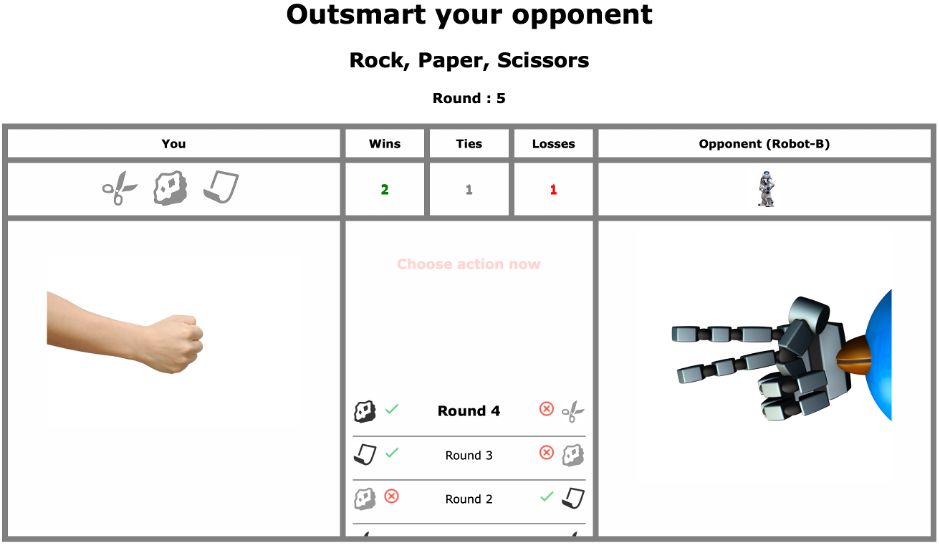
\includegraphics{../Report/images/feedback_rps} 

}

\caption{Screenshot of the feedback at the end of a round of Rock-Paper-Scissors}\label{fig:feedback-rps}
\end{figure}

To summarise, all the games used in both experiments have a unique MSNE consisting of randomising across actions. If participants follow this strategy, or simply dont engage in learning how the opponent plays, they woud score 0 on average against both level-1 and level-2 players. Evidence of sustained wins would indicate that participants have learned to exploit patterns in the opponent play.

\newpage

\hypertarget{results}{%
\section{Results}\label{results}}

\hypertarget{first-experiment-1}{%
\subsection{First Experiment}\label{first-experiment-1}}

In the first experiment, a total of 52 (28 female, 24 male) participants were recruited on the Prolific Academic platform. The mean age of participants was 31.2 years. Participants were paid a fixed fee of £2.5 plus a bonus dependent on their performance which averaged £1.06. The study used a 2 (computer opponent levels 1 and 2) by 3 (games of rock-paper-scissors, fire-water-grass and numbers) design, with repeated measures on the second factor.

Looking at the aggregate scores, the RPS game had the lowest average score across participants (M = 0.289, SD = 0.348) followed by NUMBERS (M = 0.31, SD = 0.347) and finally the FWG game had the highest average score (M = 0.454, SD = 0.354). Aggregate average scores for each game were significantly different from 0 (hypothesised value of random play) using parametric one sample t-tests (RPS: t(51) = 7.26, p-value = 2.1e-08 ; FWG: t(51) = 10.04 , p-value = 1.10e-13 ; NUMBERS: t(51) = 7.17, p-value = 2.87e-09).

To analyse within and between game learning, we used a 2 (condition: level-1, level-2) by 3 (game: RPS, FWG, NUMBERS) by 2 (block: first half, second half) repeated measures ANOVA with the first factor varying between participants. As the number of participants facing level-2 agents was slightly higher than those facing level-1 agents (28 vs 24), the ANOVA is unbalanced. We therefore used the ``afex'' (Singmann \& al., 2016) package in R, as it allows us to handle unbalanced designs and produces type III sum of squares by default.

There was a main effect of Game ( F(2,100) = 8.54, ges = 0.05, p = .0005), showing that average scores varied significantly over the games. Post-hoc pairwise comparisons showed that performance in the FWG game was significantly higher than in the RPS game ( t(100) =3.78, p = 0.0008 ), and the performance in NUMBERS was significantly lower than FWG game ( t(100) = -3.32 , p = 0.0024). The score in RPS was not significantly different from the score in NUMBERS however ( t(100) = 0.45 , p = 0.65). The main effect of Block ( F(1,50) = 22.51 , p \textless{} .001, ges = 0.03) shows that the average score in the first half of games (M = 0.29) was significantly lower than in the second half of the games played (M = 0.40), which translates to within-game learning : as players get more interaction with the agent, they learn how to win more often. The main effect of Condition (F(1,50) = 5.44, p = .024, ges = 0.05) indicates that scores were higher against the level-1 player (M = 0.43) than against the level-2 player (M = 0.27). This means that it was harder for participants, on average, to learn the strategy of the more sophisticated opponent (level-2) compared to that of the comparatively less sophisticated agent (level-1). Finally, the analysis showed a significant interaction effects of block by game ( F(2,100) = 6.92 , p = .002, ges = 0.02), indicating that within-game learning differed between the games, as well as a three-way interaction between condition, game, and block ( F(2,100) = 3.88 , p = .023, ges = 0.01).

\hypertarget{learning-transfer}{%
\subsubsection{Learning transfer}\label{learning-transfer}}

As a measure for learning transfer, we focus on participants' scores in rounds 2-6, excluding the very first round for which the agent is programmed to play randomly as it has no data on prior rounds on which to build its response. A group of players with no experience of the game are expected to have scores not significantly different from 0. Any significantly positive group average scores would therefore reflect prior learning from past experiences. In Figure~@ref(fig: exp1-early-score), the average score across participants by game for rounds 2-6 are plotted. Scores are also averaged across levels of condition.

\begin{figure}

{\centering 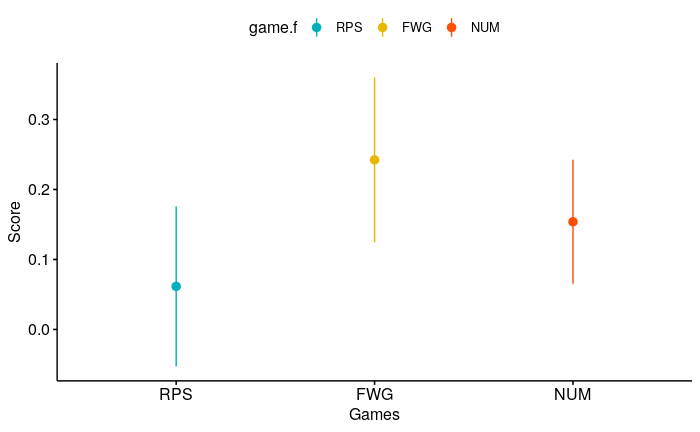
\includegraphics{../Report/images/exp1_early_scor_game} 

}

\caption{Average scores for rounds 2-6 by game in first experiment}\label{fig:exp1-early-score}
\end{figure}

We test the average scores for each game against a hypothesised value of 0 for a non-experienced player using parametric one sample t-tests. As expected for the initial RPS game, the average score is not significantly different from 0 as this is the first game and no learning is possible (t(148.85) = 1.04 , p = 0.89). In FWG, the score is significantly higher than 0 ( t(148.85) = 4.58 , p \textless{} 0.0001). This is also the case for the more dissimilar game : NUMBERS ( t(148.85) = 3.00, p = 0.0092).

Next, we explore whether learning transfer is moderated by the type of opponent and game similarity. Figure~@ref(fig: exp1-score-by-opp) shows the marginal mean scores for each game for both level-1 and level-2 facing players. Graphically we can see that the pattern is dissimilar between level-1 and level-2 players, and we suspect transfer to be positively associated with similarity and negatively with degree of sophistication of the agent. To test these hypotheses, we run statistical tests on scores by game and opponent against the null hypothesis of 0 (no transfer).

\begin{figure}

{\centering 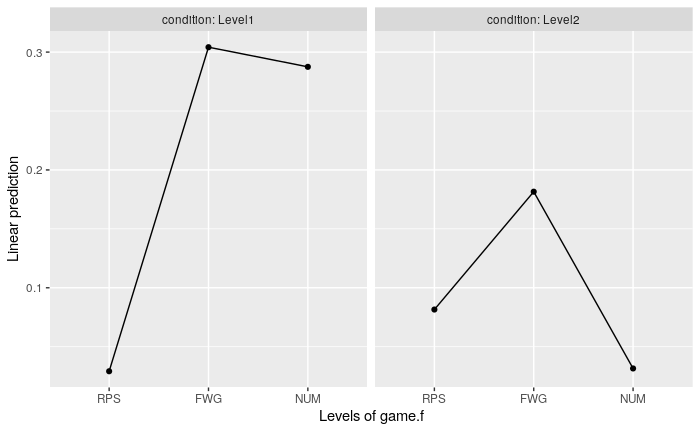
\includegraphics{../Report/images/exp1_earlyScore_by_opp} 

}

\caption{Marginal means of players scores by game and type of opponents}\label{fig:exp1-score-by-opp}
\end{figure}

Table~\ref{tab:table-early-scores} shows the scores on rounds 2-6 for both type of opponents in each game. We also report the t-stats and p-values to test the null hypothesis that scores on these early rounds are equal to 0. Rejecting the null hypothesis means that prior learning has been used to beat the opponent in these early rounds. For level-1 facing players, there is evidence of learning transfer from RPS to both FWG and NUMBERS. For level-2 facing players, there is evidence for transfer from RPS to the similar game FWG (albeit scores are lower than for level-1 player) but not to the dissimilar game of NUMBERS.

\begin{table}[tbp]
\begin{center}
\begin{threeparttable}
\caption{\label{tab:table-early-scores}Average early round scores by game and condition in first experiment}
\begin{tabular}{lllllllll}
\toprule
game.f & \multicolumn{1}{c}{condition} & \multicolumn{1}{c}{lsmean} & \multicolumn{1}{c}{SE} & \multicolumn{1}{c}{df} & \multicolumn{1}{c}{lower.CL} & \multicolumn{1}{c}{upper.CL} & \multicolumn{1}{c}{t.ratio} & \multicolumn{1}{c}{p.value}\\
\midrule
FWG & Level1 & 0.30 & 0.08 & 149.58 & 0.10 & 0.51 & 3.96 & 0.00\\
NUM & Level1 & 0.29 & 0.08 & 149.58 & 0.08 & 0.49 & 3.74 & 0.00\\
RPS & Level1 & 0.03 & 0.08 & 149.58 & -0.18 & 0.23 & 0.38 & 1.00\\
FWG & Level2 & 0.18 & 0.07 & 147.52 & -0.01 & 0.38 & 2.48 & 0.06\\
NUM & Level2 & 0.03 & 0.07 & 147.52 & -0.16 & 0.23 & 0.43 & 1.00\\
RPS & Level2 & 0.08 & 0.07 & 147.52 & -0.11 & 0.28 & 1.11 & 0.80\\
\bottomrule
\end{tabular}
\end{threeparttable}
\end{center}
\end{table}

Our results when averaging across conditions (previous section) showed that there was indeed evidence for transfer to the more dissimilar game (NUMBERS). We can see from TABLE~\ref{tab:table-early-scores} that this transfer is exclusively driven by level-1 facing players, as scores of level-2 facing players are close to nil. Therefore, both groups of condition can generalise to the similar game, but only those facing the less sophisticated opponent are able to generalise to the less similar game.

\hypertarget{second-experiment-1}{%
\subsection{Second Experiment}\label{second-experiment-1}}

A total of 48 participants (21 females, 28 males, 1 unknown) used the Prolific Academic platform to participate in the experiment. The average age of players was 30.2 years, and the mean duration to complete the task was 39 minutes. Participants were incentivised using a two-tier payment mechanism: a fixed fee of £2.5 for completing the experiment plus a performance linked bonus that averaged £1.32. The participants faced two types of opponents, a level-1 and level-2 players, and played a total of 3 games (Rock-Paper-Scissors, Fire-Water-Grass, and the Penalty Shootout game), with repeated measures on the latter factor. Each game was split into 4 stages. The players faced either the level-1 or level-2 player on the first stage, and the other opponent in stage 2, for 20 rounds in each stage. Stages 3 and 4 were repetitions of the first two stages but with only 10 rounds in each stage.

The RPS game had the lowest average score per round (M = 0.194, SD = 0.345) followed by FWG (M = 0.27, SD = 0.394) and finally the Shootout game had the highest average score (M = 0.622, SD = 0.326). The higher score in shootout is expected as there are 2 out of three possible winning actions, compared to one out of three in RPS and FWG. Indeed, a player not aiming to uncover the opponent's strategy and thus choosing to play randomly should be expected to have on average score per round of 0 in both RPS and FWG, and 0.33 in the Shootout game. To make the scores more comparable, and because we are interested in player's performance that is not due to chance, we will correct all scores in the shootout game by subtracting the average score per round of a random strategy (0.33). Using parametric t-tests on adjusted scores, we reject the null hypothesis of random play in all three games (RPS: t(49) = 6.26, p-value \textless{} 0.0001 ; FWG: t(49) = 7.25 , p-value \textless{} 0.0001 ; SHOOT: t(49) = 13.61, p-value \textless{} 0.0001 ).

Using the average scores obtained by participants in each game and interaction, we explore whether learning has occurred within and between games. We perform a two (condition: level-1 first, level-2 first) by two ( opp\_type: level\_1 or level\_2) by three (game: RPS, FWG, SHOOT) by two (interaction: first or second) repeated measures ANOVA with the first factor varying between participants. As the number of participants facing level-1 agents was slightly higher than those facing level-2 agents (27 vs 23), the ANOVA will not be balanced between the two levels of condition. We therefore used the ``afex'' (Singmann \& al., 2016) package in R, as it allows us to handle unbalanced designs and produces type III sum of squares by default. The full results of this analysis are provided in Table~\ref{tab:exp2-anova}.

\begin{verbatim}
## Warning in summary.Anova.mlm(x$Anova): HF eps > 1 treated as 1
\end{verbatim}

\begin{table}[tbp]
\begin{center}
\begin{threeparttable}
\caption{\label{tab:exp2-anova}ANOVA results for experiment 2}
\begin{tabular}{lllllll}
\toprule
Effect & \multicolumn{1}{c}{$F$} & \multicolumn{1}{c}{$\mathit{df}_1^{GG}$} & \multicolumn{1}{c}{$\mathit{df}_2^{GG}$} & \multicolumn{1}{c}{$\mathit{MSE}$} & \multicolumn{1}{c}{$p$} & \multicolumn{1}{c}{$\hat{\eta}^2_G$}\\
\midrule
Condition f & 0.45 & 1 & 48 & 0.43 & .505 & .003\\
Game f & 11.81 & 1.85 & 88.71 & 0.12 & < .001 & .039\\
Interaction lvl & 1.34 & 1 & 48 & 0.06 & .253 & .001\\
Opp type & 0.00 & 1 & 48 & 0.12 & .973 & .000\\
Condition f $\times$ Game f & 1.34 & 1.85 & 88.71 & 0.12 & .266 & .005\\
Condition f $\times$ Interaction lvl & 0.03 & 1 & 48 & 0.06 & .864 & .000\\
Condition f $\times$ Opp type & 0.13 & 1 & 48 & 0.12 & .717 & .000\\
Game f $\times$ Interaction lvl & 0.46 & 1.99 & 95.72 & 0.08 & .635 & .001\\
Game f $\times$ Opp type & 5.31 & 1.7 & 81.82 & 0.11 & .010 & .015\\
Interaction lvl $\times$ Opp type & 2.16 & 1 & 48 & 0.04 & .148 & .001\\
Condition f $\times$ Game f $\times$ Interaction lvl & 2.43 & 1.99 & 95.72 & 0.08 & .094 & .006\\
Condition f $\times$ Game f $\times$ Opp type & 1.23 & 1.7 & 81.82 & 0.11 & .294 & .003\\
Condition f $\times$ Interaction lvl $\times$ Opp type & 0.02 & 1 & 48 & 0.04 & .883 & .000\\
Game f $\times$ Interaction lvl $\times$ Opp type & 0.96 & 1.89 & 90.83 & 0.09 & .383 & .002\\
Condition f $\times$ Game f $\times$ Interaction lvl $\times$ Opp type & 0.94 & 1.89 & 90.83 & 0.09 & .390 & .002\\
\bottomrule
\end{tabular}
\end{threeparttable}
\end{center}
\end{table}

There is evidence for a main effect of Game on scores (F(1.85,88.7) = 11.81, ges = 0.04, p \textless{} .0001), meaning that we reject the null hypothesis of scores in games being equal. To explore these differences further, we look at post-hoc analyses for pairwise comparisons between game scores (p-values adjusted using Holm method for multiple comparisons). We find the performance in the games increases steadily throughout the experiment, with FWG performance significantly higher than RPS (t(96) =2.53, p = 0.025), and performance in the SHOOT game also significantly higher than in FWG ( t(96) = 2.32, p = 0.025 ). There was no main effect of either opponent type, the interaction factor( first or second time opponent was faced) , or the condition factor (whether level-1 or level-2 opponent was faced first). This means that neither the type of opponent faced, nor whether it was the first or second interaction with the opponent nor which opponent was faced first did have a main effect on performance.

\hypertarget{learning-transfer-1}{%
\subsubsection{Learning transfer}\label{learning-transfer-1}}

As a measure for learning transfer we will compare scores only on the first 5 rounds (rounds 2-6 of each game, excluding the very first round where play is necessarily random). Because the number of rounds here is very limited, there should be very little learning within games, and we should be better measure learning transfer if it exits.

\begin{figure}

{\centering 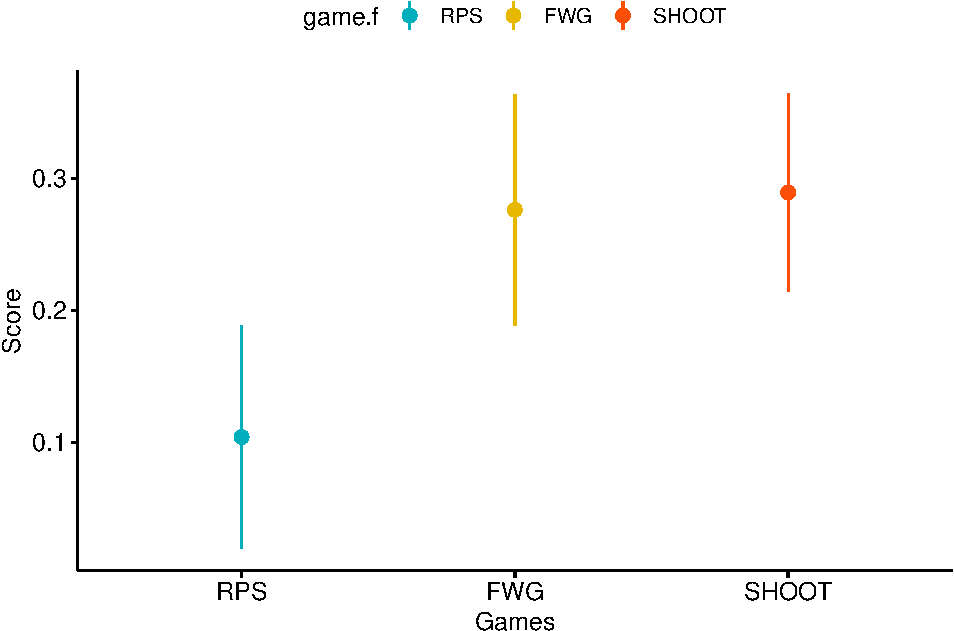
\includegraphics{draft_report_v1_files/figure-latex/exp2-early-scores-1} 

}

\caption{Average early round scores by game for experiment 2}\label{fig:exp2-early-scores}
\end{figure}

In Figure~\ref{fig:exp2-early-scores}, we show the average score across participants in rounds 2-6 of the first interaction with the opponent for each game. These scores are also averaged across the levels of condition (meaning they are irrespective of which opponent players faced first). For both the FWG and SHOOT games, score in the early rounds of the first interaction are significantly higher than 0 for both opponent types. (Level-1 opponent: FWG: t(270) = 4.99, p \textless{} 0.0001; SHOOT: t(270) = 6.66, p \textless{} 0.0001; Level-2 opponent: FWG: t(270) = 4.40, p \textless{} 0.0001; SHOOT: t(270) = 3.21, p =0.004 ). Looking more specifically at early scores by type of opponent faced, we confirm the result from the first experiment that it is easier to transfer learning to the more dissimilar game (Shoot) when facing a level 1 opponent. Indeed, while the early scores of FWG for level-1 and level-2 facing players are not significantly different from each other, the score of the players facing the level-1 opponent is indeed almost 0.2 point per round higher than that of players facing level-2 opponents, and the difference is statistically significant ( t(144) = 2.45 , p = 0.01). These early scores have also been adjusted to account for the fact that the shootout game has higher average scores when playing randomly, and therefore this difference is really due to better learning transfer and not due to chance.

\newpage

\hypertarget{computational-modelling}{%
\section{Computational modelling}\label{computational-modelling}}

To gain more insight into how participants played the games against the computer opponents, we compared multiple models of strategies the players may have been using to learn how to beat the opponent. As a base model, we assume play is random, and each potential action is chosen with equal probability. Note that this corresponds to the Nash equilibrium strategy. Next, we include for comparison purposes a few other basic models of behavior, such as Q-learning on action choices, as well as a more sophisticatd Q-learning model incorporating a state space consisting of last round play. The Bayesian approach is represented by models whereby agents would update an initial belief over the opponent's strategy consisting of various level-k strategies (resp. 0,1 and 2). We fitted two models in which agents best respond to the opponent model. In the first, the beliefs about the opponent's adopted strategy are transfered across games, and another in which no transfer of opponent models is allowed.

Next, we fitted a self-tuning EWA model (Ho et al., 2004) both on action choices without states and with states consisting of lat round play. The self-tuning EWA model generalizes both reinforcement learning as well as fictitious play models and has been proven to do well than equilibrium models in various game situations. Finally, we also included a model-based reinforcement learning approach. whereby the agent learns the transition probabilities between states ans uses that to choose the best action, given the current state and it's belief about what the new state will be.

All models were fit to each participant in both experiments, with optimal parameters being estimated using maximum likelihood. Using information criteria based Bayesian model comparison (BIC), the best fitting model for each participant was chosen and we compared the number of participants whose behavior was explained by each model. Figure~\ref{fig:exp1-comp-models} shows the results for experiment 1: we can see that while some participant's learning behavior was either random or explained by some of the base models, a significant number of participants in experiment one had learning most consistent with Q-learning conditional on last round play.

\begin{figure}

{\centering 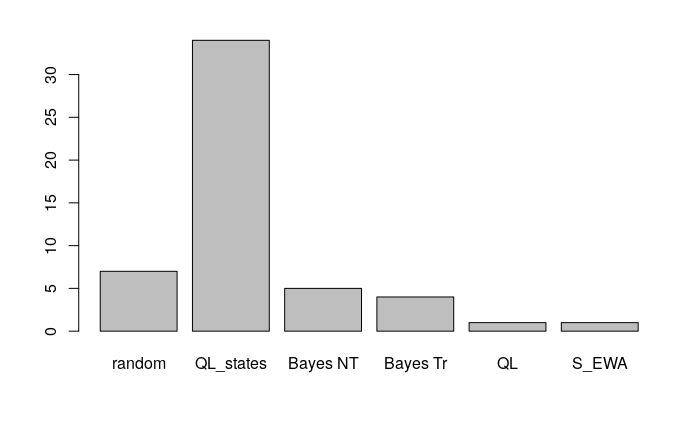
\includegraphics{../Report/images/exp1_comp_models} 

}

\caption{Histogram of best fitting computational models for experiment 1}\label{fig:exp1-comp-models}
\end{figure}

In experiment 2 however, we can see from Figure~\ref{fig:exp2-comp-models} that Q-learning with the aforementioned state-space wasn't as successful as the bayesian approached in fitting player's action choices. In experiment 2 when participants faced both level-1 and level-2 agents sequentially, the bayesian models (with or without transfer) were by far the most successful.

\begin{figure}

{\centering 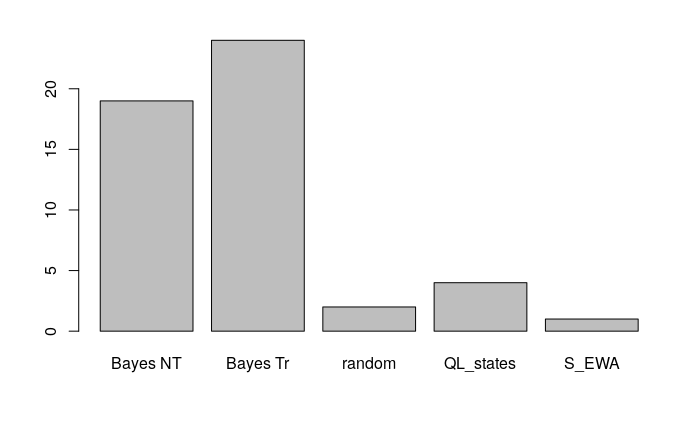
\includegraphics{../Report/images/exp2_comp_models} 

}

\caption{Histogram of best fitting computational models for experiment 2}\label{fig:exp2-comp-models}
\end{figure}

Next we compared the performance of players whose actions are consistent with each of our hypothesized models. Figure~\ref{fig:exp1-cumScores} shows the average cumulative performance of players across games, for participants grouped by which model best fits their behavior in experiment 1. We can see that participants whose actions are most consistent with learning an opponent model in a Bayesian way had the best overall performance (both with and witout transfer), followed by Q-learning conditional on last round play. EWA, QL and random players had, understandably the lowest performance.

\begin{figure}

{\centering 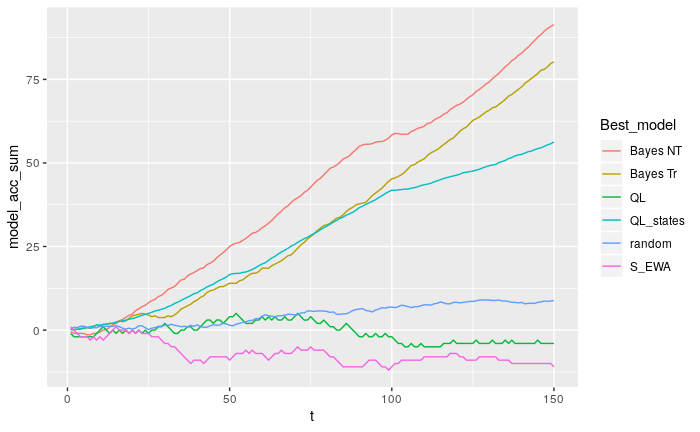
\includegraphics{../Report/images/exp1_cumScores} 

}

\caption{Average cumulative scores of participants in experiment 1 by best fitting model}\label{fig:exp1-cumScores}
\end{figure}

Doing the same exercise for experiment 2, we see very similar results looking at Figure~\ref{fig:exp2-cumScores}, in that participants whose behavior was best fit by a bayesian model of learning the oppponent strategy had the highest cumulative performance, followed by theose relying on reinforcement learning with a state space of last round play, and as expectedm random play as well as EWA were at the bottom of cumulative performance.

\begin{figure}

{\centering 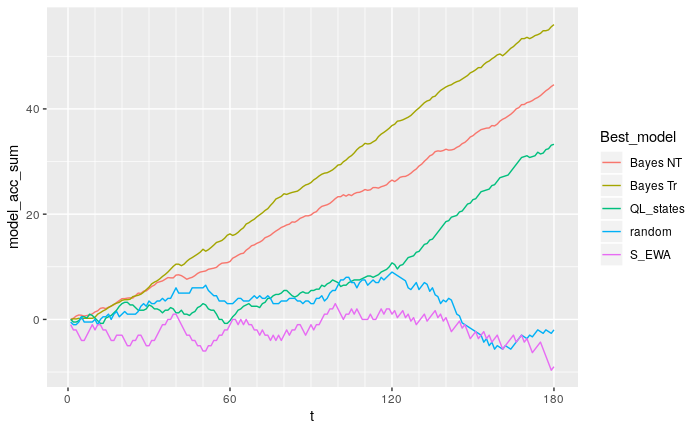
\includegraphics{../Report/images/exp2_cumScores} 

}

\caption{Average cumulative scores of participants in experiment 2 by best fitting model}\label{fig:exp2-cumScores}
\end{figure}

\newpage

\hypertarget{discussion}{%
\section{Discussion}\label{discussion}}

In this study, we investigated human learning transfer across games by making human participants play against computer agents with rule-based level-k strategies. We were interested in uncovering evidence for transfer and exploring whether it is modulated by the degree of similarity between games and the sophistication of the agent.

The results of our first online experiment show that the majority of participants learn to adapt to the opponent strategy over multiple interactions and generalise this learning to the similar game. We found that using results on very early rounds is a better proxy for measuring transfer as it is not tainted by any within game learning. Using this approach, we showed that transfer to the more dissimilar game was modulated by the degree of sophistication of the agent, with evidence for transfer when players face the less sophisticated agent but not the more sophisticated one.

In the second online experiment, the paradigm was better suited to explore our main research question, related to learning transfer rather than within-game learning. Indeed, when facing two opponents sequentially, there are many more opportunities to test transfer than before. Indeed, there are 2 opportunities to transfer knowledge within each game, and a total of three games, which means 6 opportunities to test transfer. When we made players face only one type of opponent each, we only had two possible learning transfers to test. In that regard, the results on learning transfer confirmed prior findings from the first experiment. While there was no evidence of learning transfer across interactions within the same game (likely due to the lower number of rounds per interaction and the higher cognitive load of facing two opponents rather than one), we found evidence for learning transfer across games as early round scores analysis confirmed. We also found that learning transfer is modulated by the type of opponent faced. When the players faced the level-1 opponent, they were able to transfer learning. However, when they faced the level-2 opponent, there was weaker evidence for transfer. The lack of transfer when facing the more sophisticated opponent might be due to the difficulty of learning that opponent strategy to start with. A player cannot transfer what they have not learnt and as such, since it might be harder to learn the strategy of the level-2 opponent, this in turn might translate into weaker evidence for transfer.

Coming back to evidence for learning transfer, we observed evidence that participants start off new games with prior knowledge as their scores are much higher than chance, confirmed both by early stage analysis as well as rounds 2-6 scores analysis. The question we ask ourselves therefore is: What exactly did the players learn in RPS that allowed them to beat the opponent in FWG and SHOOT? what did the players learn exactly about the opponent strategy and what form did this learning take?

We will proceed by considering multiple potential answers to this question. First, maybe players simply learn spatial heuristics that allow them to perform better than chance. An example is a spatial heuristic that consists of choosing ``weapons'' in a particular order (for instance left to right). This was one of the weaknesses in the design of experiment one, as it was indeed possible using very simple spatial sequences to beat the opponent on most rounds. We took this into account in designing experiment two by randomly shuffling the spatial order of action choices in each round. Still, the learning and conclusions were similar, so this could not explain both learning and transfer in experiments one and two.

A second possible hypothesis for learning the opponent's strategy is the use of simple rules based on last round play (for instance, I play scissors whenver opponent played rock in last round, or whenever the last round play was rock/scissors, I should play paper in this round, etc\ldots{}). Our Q-learning with states as prior-round play model is a good proxy for this type of strategies. While this approach certainly seemed to be the best fit for some player's behavior, it is unsatisfactory in explaining some of the learning transfer evidence we showed. Indeed, learning the best action in a particular state cannot easily transfer to a new game since the state space is different and there is no simgle mapping between the state spaces of the initial and latter games. These rules would thereofre need to be learned anew in the latter game which is inconsistent with above chance performance in very early rounds.

Likewise, assuming that players learn a complete model of the environment (for instance the transition probabilities from last round play to new play) might explain learning within games but is equally unable to account for early games transfer of learning as such models, besides being cognitively very expensive to learn, would require many rounds of practice. Another issue with these hypotheses is that they are not consistent with significant score differences between those facing level-2 and level-1 opponents. After all, if players were using some type of associative learning or spatial heuristics, then their scores should not depend on the degree of strategic sophistication of the opponent since their approaches would render this variable irrelevant. The fact that the degree of sophisitication of the opponent matters points to the importance of opponent modelling to successful transfer of learning.

We are left with two possible explanations: First, it is possible that the players have uncovered a heuristic that allows them to beat the opponent without explicitly modelling their strategy, and is robust to transfer. Indeed, because of the cyclicality in action choices (e.g : Rock beats Scissors beats Paper beats Rock), it is possible to beat level-2 opponents most of the time by following a simple rule: Play in the next round whatever the opponent played in the last round. This is a rule that wins and is also robust to transfer as it does not depend on action labels and even works in the dissimilar game.

The second explanation of learning transfer is that it is driven by a group of participants that are able to build a mental representation of what the strategy of the opponent is. A successful mental representation would take the perspective of the opponent or endow it with intentionality in order to detect its strategy when the opponent is playing based on a level-k reasoning model. For instance, the player may think ``My opponent is always trying to be one step ahead of me, therefore, I will be one step ahead of where it thinks I will be''. This mental representation would facilitate the use of theory of mind abilities and thus enable the players to learn opponent strategies when they are based on human-like reasoning models such as level-k or cognitive hierarchy. This type of learning would be deemed ``explicit'' in the psychology literature as a process through which knowledge consists of cognitive representations of concepts and rules, as well as the relationship between them. It involves the evaluation of explicit hypotheses and results in better problem-solving skills (Mandler, 2004). Since it is less context dependent, this type of learning is generalizable to new situations, akin to the more general framework of rule-based learning explored by Stahl (2000, 2003).

Our second experimental design allows us to test whether the first explanation holds. Since there is a simple transferable heuristic that works agaisnt level-2 players, and since as far as we know, there are no similar ones against level-1 players, if indeed participants were using this, they would perform better and transfer learning more easily when facing level-2 opponents. Because level-2 opponents use a higher level of strategic reasoning, they should in fact be harder to play against and in the absence of such a heuristic, performance and learning transfer should be worse.

Our results show that in fact, it was harder to transfer learning when facing level-2 opponents, both comparing first intractions across games and using early rounds analysis. Based on our assumptions, we conclude that the most likely explanation is that participants who are able to beat the opponent and transfer learning are likely to be explicitly modelling the opponent strategy using level-k reasoning, compared to using simple learning rules they uncovered during the ourse of learning.

\newpage

\hypertarget{conclusion}{%
\section{Conclusion}\label{conclusion}}

Our online experiments confirm behavioural game theory results, stating that human players can deviate from Nash equilibrium play and learn to adapt to the opponent strategy and exploit it when the opponent itself is deviating from Nash equilibrium. Moreover, we showed that participants do transfer their learning to new games with varying degrees of similarity. The most likely explanation as we saw is that players build a mental representation of their opponent strategy, rather than rely on associative learning or action-based heuristics. The transfer is also moderated by the level of sophistication of the opponent, with participants showing more success in learning and transferring against opponents adopting a less sophisticated strategy.

Having said that, there remains a high degree of heterogeneity between players. There is a high positive association between players who learn to beat the sophisticated and less sophisticated opponents, indicating that some players are more able to detect the patterns in opponent play and learn how to exploit them. Moreover, the computational modelling shows that a significant number of players are still using random strategies in the games. Whether this ability depends on engagement with the experiment or on other characteristics of the learner is an open question that more research in the area would hope to answer.

\newpage

\hypertarget{references}{%
\section{References}\label{references}}

\begingroup
\setlength{\parindent}{-0.5in}
\setlength{\leftskip}{0.5in}

\hypertarget{refs}{}
\leavevmode\hypertarget{ref-lakeBuildingMachinesThat2017}{}%
Lake, B. M., Ullman, T. D., Tenenbaum, J. B., \& Gershman, S. J. (n.d.). Building machines that learn and think like people. \emph{Behavioral and Brain Sciences}, \emph{40}. \url{https://doi.org/10.1017/S0140525X16001837}

\endgroup

\end{document}
